\subsection{Data Processing and Mixed Precision Training}
\label{back:data}

\subsubsection{Data Normalization}

Normalization is a technique by which data is transformed from its original scale to a more standard scale \cite{ali2014data}. These techniques are normally used when the dataset has elements of different ranges. Normalization can contribute to faster convergence, and it's why they are as commonly used when preprocessing data. 

\textbf{MinMax Normalization} 

This algorithm transforms data to a specified range, most often $[0, 1]$, but it can also be $[-1, 1]$ or any other range.
The minmax normalization function can be formulated as follows:
\begin{equation}
   x_{\text{normalized}} = \dfrac{x - x_{min}}{x_{max}-x_{min}}
\end{equation}
\vspace{0.2cm}
where $x$ denotes the data, $x_{min}$ and $x_{max}$ is the minimum and maximum in $x$. \\
%
\subsubsection{Half-Precision and Mix-Precision Training}

Working with large datasets and \acrshort{dnn}s can be rather time- and resource-consumptive. One can cast the datatype from single precision to half-precision, along with weights, biases, and losses to address this. This will reduce the loss of accuracy and information, but it can drastically lower memory consumption and decrease training time. It is important to note that datacasting occurs with normalization techniques; the order in which the operation happens first is quintessential. If the data is cast to half precision before normalization, the normalization will be based on a slightly inaccurate representation of the data, but the computation of the normalized data will be faster. If normalization were to occur first, less detail about the data would be lost, but at the expense of being more computational intensive.\\

\begin{figure}[!h]
    \centering
    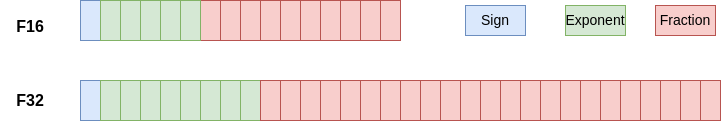
\includegraphics[width=0.8\linewidth]{figures/floats.png}
    \caption{Float16 have a limited amount of bits to represent floating point numbers compared to Float32}
    \label{fig:floats}
\end{figure}

To combat vanishing- or even exploding gradients, we can instead do some operation in \texttt{Float32} while others in \texttt{Float16}. Mixed precision training, introduced in 2018 \cite{micikevicius2018mixed}, is a technique where a neural network's weights, activations, and biases are stored in single precision while the data stays in its original format. It allows for reduced memory consumption while also speeding up the operations of deep neural nets. Additionally, the amount of $\si{\kilo\watt\hour}$ required to train the neural nets would decrease, thus reducing both the cost and the environmental tax of training neural nets. This becomes more important with larger datasets, models, and the sheer amount of GPUS required to train massive workloads. This introduces the concept of loss scaling, where the losses must be adjusted based on the weights. \\

\mycomment{
\subsection{Dataloaders}

If the datasets contain information about the data and how to retrieve a single instance, the dataloaders job is to create an object that can be iterated over, containing $n$ amount of batches, and transferring these data to the wanted devices. In the case of data parallel multi-gpu training, when the data is loaded, it's \textit{sharded} across the different gpus, in a manner that balances the load of each gpu. Let's say we have a batch  of size $[4, 5, 5]$ and we have two gpus available. The dataloader can split this Tensor in two batches, where each of the gpus get a tensor of size $[2, 5, 5]$. By sharding the data along the first axis, ideally we can half the amount it takes, not taking data transfer time into consideration. 

\begin{figure}[!h]
    \centering
    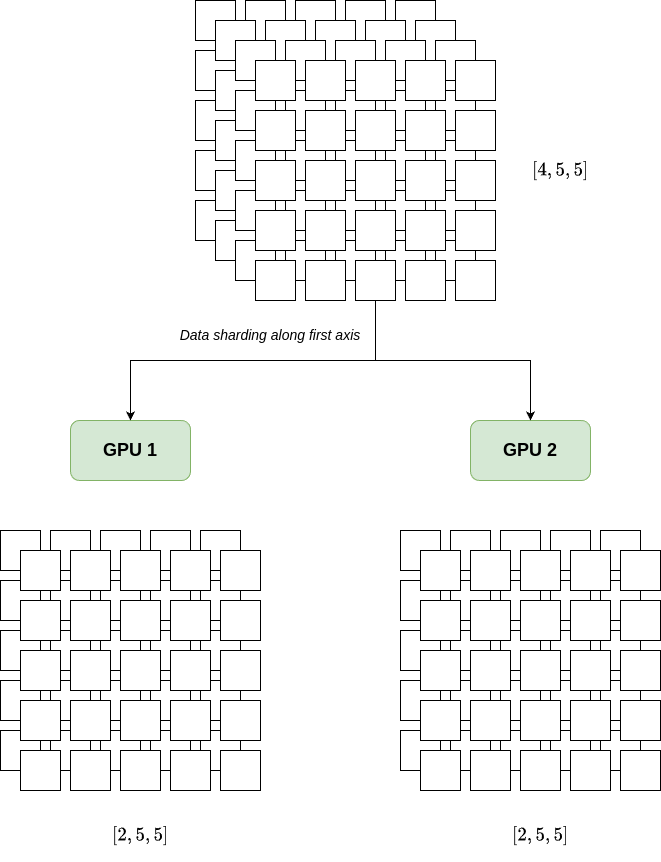
\includegraphics[scale=0.4]{figures/sharding.png}
    \caption{Example of data sharding with 2 gpus, and a original Tensor of size [4,5,5]}
    \label{fig:sharding}
\end{figure}


\textbf{Parallel loading}

When iterating over a dataloader, each element of the batch is retrieved and undergoes transformations. Depending on the batch size and  the size of the data, this procedure can be very resource-intensive and time-consuming. To mitigate this, we can introduce the concept of parallel batch loading. Instead of gathering and transforming the data sequentially, one can leverage available resources to do this operation in a parallel manner. Algorithm \ref{alg:parallel-batch-loading} details how such an operation is conducted.


\begin{algorithm}
\caption{Parallel Batch Data Loading}\label{alg:parallel-batch-loading}
\begin{algorithmic}
\Require BatchIndices, N
\Ensure BatchData, LoadSingleData
\State Initialize empty list BatchData
\State Create ThreadPool with N threads
\For{each Index in BatchIndices}
    \State Submit LoadSingleData(Index) to executor
\EndFor
\For{each completed Future from executor}
    \State Data $\gets$ Future.result()
    \State Append Data to BatchData
\EndFor
\State \Return BatchData
\end{algorithmic}
\end{algorithm}
}

\subsubsection{Overfitting and Early Stopping}

Overfitting is a common problem within \acrlong{ml} \cite{srivastava2014dropout}. It occurs when a model is trained to close to the training data, and fails to capture features of other data.In addition to popular techniques such as dropout \cite{srivastava2014dropout}, \textit{early stopping} is a regularization technique that aims to avoid overfitting. When training an optimizer such as \acrshort{adam} \cite{kingma2017adam}, or \acrshort{sgd} , one can notice when a model is overfitting by studying the validation loss. If the validation loss $L_v$ starts increasing, the early stop mechanism will stop the training altogether if no improvement of $L_v$ by at least $\epsilon$ is found after $p$ number of epochs. This can described accordingly; we stop at epoch $T$ if:
\begin{equation}
\forall i \in \{T-p+1, ..., T\}: L_v(i) > L_v^* - \epsilon
\end{equation}
where $L_v^*$ is defined as:
\begin{equation}
L_v^* = \min_{j=1}^{T} L_v(j)
\end{equation}

\subsubsection{Parallelism within \acrlong{dl}}

With rapidly evolving deep learning architectures and workloads, the importance of scalable training grows each year. It is estimated that these networks grow $\qty{1.5}{x}$ each year \cite{9499913}, making parallelization a vital topic in \acrshort{ai} to accommodate ever-increasing memory needs. Several different hardware accelerators have been created to best accommodate these needs; the most apparent of these are \acrshort{gpu}s. By workers, we mainly refer to \acrshort{gpu}s, but this could also be other types of hardware accelerators such as TPUs \cite{jouppi2023tpu}.



\subsubsection{Data Parallelism}

Data parallelism refers to partitioning data across multiple workers. Given a dataset $X$, we can split $X$ across the workers and store a copy of the model $M$ on each worker, calculate gradients across them all and update the trainable parameters for $M$ Example of how data can. 

\begin{figure}[!h]
    \centering
    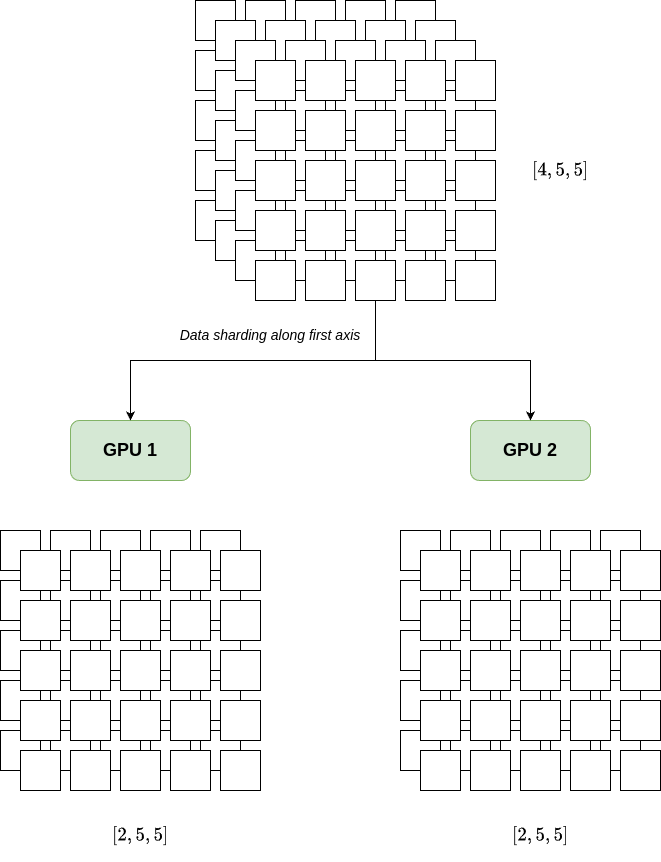
\includegraphics[width=0.7\linewidth]{figures/sharding.png}
    \caption{Example of data parallel training, where a tensor $M$ of dimensions $[4,5,5]$ is split on the first axis across two \acrshort{gpu}s, leading to each \acrshort{gpu} receiving a tensor of dimension $[2,5,5$.}
    \label{fig:dataparallel}
\end{figure}

